\section{Non-crossing 2-partitions}

\begin{definition}[Non-crossing 2-partition]
    A \emph{non-crossing 2-partition} of a \emph{totally
    ordered} set $E$ is a pair $(P, \sigma)$
    where :\\
    \begin{itemize*}
        \item $P$ is a non-crossing partition of $E$\\
        \item $\sigma$ is a permutation of the elements of $E$\\
        \item For each \emph{sorted} block
            $B_i = \{b_1, \ldots, b_k\} \in P$, we have
            $\sigma (b_i) < \ldots < \sigma (b_k)$\\\\
    \end{itemize*}
    We denote by $\mathcal{NC}^2_n$ the set of non-crossing
    2-partitions of $[n]$.
    $$\mathcal{NC}^2 = \bigcup_{n > 0}{\mathcal{NC}^2_n}$$.
\end{definition}

\begin{example}[$\mathcal{NC}^2_6$]
    \begin{itemize*}
            \subitem $P = \{\{1, 6\}, \{2, 3, 5\}, \{4\}\}$
            \subitem $\sigma = 413265$ \\
            \subitem $\hspace{36mm} \rho = \{\{1, 3, 6\}, \{2\}, \{4, 5\}\}$
    \end{itemize*}    
\end{example}

\begin{theorem}
    Let $nc^2_n$ be the cardinal of $\mathcal{NC}^2_n$.
    We have $$nc^2_n = (n + 1)^{n-1}$$
\end{theorem}

\begin{example}[$n = 1, 2, 3$]
    ~\\
    \begin{itemize}
            \item $n = 1$ \  $:$ \  $nc^2_1 = 1$
            \subitem $\{\{1\}\}$ \hspace{1cm} $1$
                \hspace{1cm} $\rho = P$
            \item $n = 2$ \  $:$ \  $nc^2_2 = 3$
            \subitem $\{\{1\}, \{2\}\}$ \hspace{1cm} $12$
                \hspace{1cm} $\rho = P$
            \subitem $\{\{1\}, \{2\}\}$ \hspace{1cm} $21$
                \hspace{1cm} $\rho = P$
            \subitem $\{\{1, 2\}\}$ \hspace{14mm} $12$
                \hspace{1cm} $\rho = P$
            \item $n = 3$ \  $:$ \  $nc^2_3 = 16$
            \subitem $\{\{1\}, \{2\}, \{3\}\}$ \hspace{1cm}
                $123$ \hspace{1cm} $\rho = P$
            \subitem $\{\{1\}, \{2\}, \{3\}\}$ \hspace{1cm}
                $132$ \hspace{1cm} $\rho = P$
            \subitem $\{\{1\}, \{2\}, \{3\}\}$ \hspace{1cm}
                $213$ \hspace{1cm} $\rho = P$
            \subitem $\{\{1\}, \{2\}, \{3\}\}$ \hspace{1cm}
                $231$ \hspace{1cm} $\rho = P$
            \subitem $\{\{1\}, \{2\}, \{3\}\}$ \hspace{1cm}
                $312$ \hspace{1cm} $\rho = P$
            \subitem $\{\{1\}, \{2\}, \{3\}\}$ \hspace{1cm}
                $321$ \hspace{1cm} $\rho = P$       
            \subitem $\{\{1, 2\}, \{3\}\}$ \hspace{14mm}
                $123$ \hspace{1cm} $\rho = P$
            \subitem $\{\{1, 2\}, \{3\}\}$ \hspace{14mm}
                $132$ \hspace{1cm} $\rho = \{\{1, 3\}, \{2\}\}$
            \subitem $\{\{1, 2\}, \{3\}\}$ \hspace{14mm}
                $231$ \hspace{1cm} $\rho = \{\{1\}, \{2, 3\}\}$
            \subitem $\{\{1\}, \{2, 3\}\}$ \hspace{14mm}
                $123$ \hspace{1cm} $\rho = P$
            \subitem $\{\{1\}, \{2, 3\}\}$ \hspace{14mm}
                $213$ \hspace{1cm} $\rho = \{\{1, 3\}, \{2\}\}$
            \subitem $\{\{1\}, \{2, 3\}\}$ \hspace{14mm}
                $312$ \hspace{1cm} $\rho = \{\{1, 2\}, \{3\}\}$
            \subitem $\{\{1, 3\}, \{2\}\}$ \hspace{14mm}
                $123$ \hspace{1cm} $\rho = P$
            \subitem $\{\{1, 3\}, \{2\}\}$ \hspace{14mm}
                $132$ \hspace{1cm} $\rho = \{\{1, 2\}, \{3\}\}$
            \subitem $\{\{1, 3\}, \{2\}\}$ \hspace{14mm}
                $213$ \hspace{1cm} $\rho = \{\{1\}, \{2, 3\}\}$  
            \subitem $\{\{1, 2, 3\}\}$ \hspace{18mm}
                $123$ \hspace{1cm} $\rho = P$\\
    \end{itemize}
\end{example}

\begin{prop}
    This means we can create a \emph{bijection} between
    $\mathcal{PF}_n$ and $\mathcal{NC}^2_n$.
\end{prop}

\begin{proof}
    ~\\
\begin{itemize}
    \item $\mathcal{PF}_n \to \mathcal{NC}^2_n$ :
    Let $f = (a_1, \ldots, a_n) \in \mathcal{PF}_n$
    be our parking function.
    For $i \in \{1, \ldots, n\}$, we define :
        \subitem $l_i$ : the number of occurences of $i$ in $f$. 
        \subitem $im_i$ : $\{j\ |\ a_j = i\}$\\
    The corresponding non-crossing partition will
    have the following constraints :
        \subitem For each $i \in \{1, \ldots, n\}$, if $l_i > 0$,
        then there is a block $B_{[i]}$ of length
        \subitem $l_i$ with minimum element $i$.
        \subitem $\sigma (B_{[i]}) = im_i$\\
    There is a unique set partition
    $\displaystyle P = \bigcup_{i}{B}_{[i]}$ of $[n]$
    and a unique permutation $\sigma$ respecting these
    conditions such that $(P, \sigma) \in \mathcal{NC}^2_n$ :
    for each minimum $i$ in \emph{decreasing order}, add
    the $n_i$ first free elements of
    $[i+1, i+2, \ldots, n, 1, \ldots, i-1]$ to $B_i$.
    $\sigma$ is then trivially obtained by the second
    constraint. 
    \item $\mathcal{NC}^2_n \to \mathcal{PF}_n$ :
    Let $(P, \sigma)$ with $P = \{B_1, \ldots, B_l\}$ be our
    non-crossing 2-partition.
    For each block $B_i = \{b_1, \ldots, b_k\} \in P$ :
    \subitem $m_i = min (B_i) = b_1$
    \subitem $pos_i = \sigma (B_i)$
    \subitem For each $j \in pos_i$, we define $a_j = m_i$\\
    The corresponding parking function is $(a_1, \ldots, a_n)$.
\end{itemize}
\end{proof}

\begin{example}[$n = 8$]
    \begin{align*}
        &P = \{\{1, 2, 5\}, \{3, 4\}, \{6, 8\}, \{7\}\}\\
        &\sigma = 36187245\\
        &f = (3, 6, 1, 7, 6, 1, 1, 3)\\
    \end{align*}
\end{example}

\subsection{The non-crossing 2-partitions poset}

\begin{definition}[$\succ^2$]
    We say that $(P, \sigma)$ covers $(Q, \tau)$, written
    ($P, \sigma) \succ^2 (Q, \tau)$,
    if $\exists B_i, B_j \in P$ such that\\
    \begin{itemize*}
        \item $Q = P - \{B_i, B_j\} \cup \{B_i \cup B_j\}$\\
        \item $l \neq i, j \and b \in B_l \rightarrow
            \tau (b) = \sigma (b)$\\
        \item Let $B_i \cup B_j = \{b_1, \ldots, b_k\}$ :\\
            \subitem $\tau (B_i \cup B_j) = \sigma (B_i \cup B_j)$\\
            \subitem $\tau (b_1) < \ldots < \tau (b_k)$
    \end{itemize*}    
\end{definition}

\begin{example}
    ~\\
    \begin{itemize*}
        \item $P = \{\{1, 6\}, \{2, 3\}, \{4\}, \{5\}\}$\\
        \item $\sigma = 236154$\\
        \item $Q = \{\{1, 6\}, \{2, 3, 5\}, \{4\}\}$\\
        \item $\tau = 235164$\\
        \item $(P, \sigma) \succ^2 (Q, \tau)$\\
        \item $(P, \sigma) \not \succ^2 (Q, \sigma)$,
        because  $\sigma (\{2, 3, 5\}) = \{3, 6, 5\}$ is
        \emph{not} ordemagenta. 
    \end{itemize*}
\end{example}

\begin{prop}
    This covering relation defines the \emph{poset} of
    $\mathcal{NC}^2_n$.
\end{prop}

\begin{rem}
    The bottom element of this poset is 
    $(\{\{1, \ldots, n\}\}, 12 \ldots n)$, and the top
    elements are $\{(\{\{1\}, \ldots, \{n\}\}, \sigma)\ 
    |\ \sigma \in \mathfrak{S}_n\}$.
\end{rem}

\begin{example}[The poset of $\mathcal{NC}^2_3$]
    ~\\
    To shorten labels, we represent
    $(\{\{1, 3\}, \{2\}\}, 213)$ by \\
    \begin{center}
        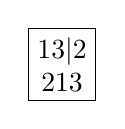
\begin{tikzpicture}
            \node (0) at (0,0) [align = center]
            [rectangle, draw]{$13|2$\\$213$};
        \end{tikzpicture}
    \end{center}

    \begin{center}
        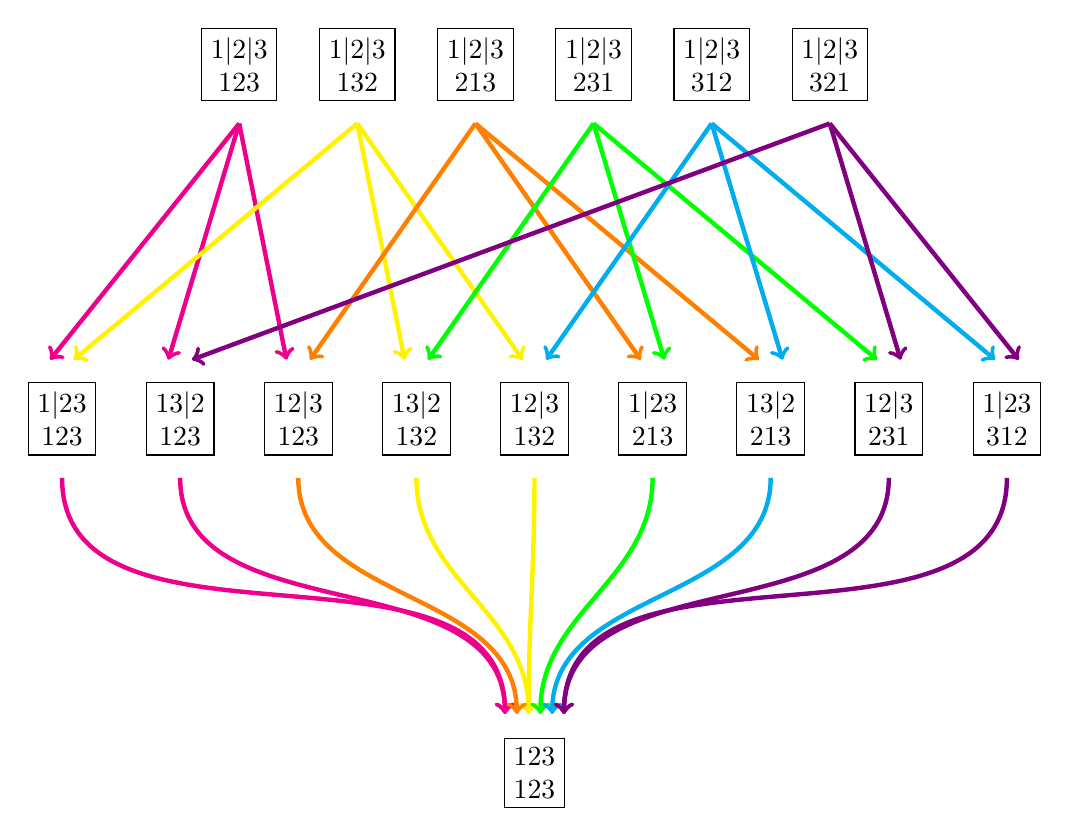
\begin{tikzpicture}[scale = 0.75]
    \node (0)  at (0,0) [align = center]
    [rectangle, draw]
        {$123$\\$123$};
    \node (1)  at (-8,6)[align = center]
    [rectangle, draw]
        {$1|23$\\$123$};
    \node (2)  at (-6,6) [align = center]
    [rectangle, draw]
        {$13|2$\\$123$};
    \node (3)  at (-4,6) [align = center]
    [rectangle, draw]
        {$12|3$\\$123$};
    \node (4)  at (-2,6) [align = center]
    [rectangle, draw]
        {$13|2$\\$132$};
    \node (5)  at (0,6) [align = center]
    [rectangle, draw]
        {$12|3$\\$132$};
    \node (6)  at (2,6) [align = center]
    [rectangle, draw]
        {$1|23$\\$213$};
    \node (7)  at (4,6) [align = center]
    [rectangle, draw]
        {$13|2$\\$213$};
    \node (8)  at (6,6) [align = center]
    [rectangle, draw]
        {$12|3$\\$231$};
    \node (9)  at (8,6) [align = center]
    [rectangle, draw]
        {$1|23$\\$312$};
    \node (10) at (-5,12) [align = center]
    [rectangle, draw]
        {$1|2|3$\\$123$};
    \node (11) at (-3,12) [align = center]
    [rectangle, draw]
        {$1|2|3$\\$132$};
    \node (12) at (-1,12) [align = center]
    [rectangle, draw]
        {$1|2|3$\\$213$};
    \node (13) at (1,12) [align = center]
    [rectangle, draw]
        {$1|2|3$\\$231$};
    \node (14) at (3,12) [align = center]
    [rectangle, draw]
        {$1|2|3$\\$312$};
    \node (15) at (5,12) [align = center]
    [rectangle, draw]
        {$1|2|3$\\$321$};

    \draw [->][color=magenta, ultra thick]
        (-5,11) to (-8.2,7);
    \draw [->][color=magenta, ultra thick]
        (-5,11) to (-6.2, 7); 
    \draw [->][color=magenta, ultra thick]
        (-5,11) to (-4.2,7);
    \draw [->][out=-90,in=90, ultra thick] 
        [color=magenta](-8,5) to (-0.5,1);
    \draw [->][out=-90,in=90, ultra thick] 
        [color=magenta](-6,5) to (-0.5,1);

    \draw [->][color=yellow, ultra thick]
        (-3,11) to (-7.8,7);
    \draw [->][color=yellow, ultra thick]
        (-3,11) to (-2.2,7);
    \draw [->][color=yellow, ultra thick]
        (-3,11) to (-0.2, 7);
    \draw [->][out=-90,in=90, ultra thick] 
        [color=yellow](-2,5) to (-0.1,1);
    \draw [->][out=-90,in=90, ultra thick] 
        [color=yellow](0,5) to (-0.1,1);
    
    \draw [->][color=orange, ultra thick]
        (-1,11) to (1.8,7);
    \draw [->][color=orange, ultra thick]
        (-1,11) to (3.8,7);
    \draw [->][color=orange, ultra thick]
        (-1,11) to (-3.8,7);
    \draw [->][out=-90,in=90, ultra thick] 
        [color=orange](-4,5) to (-0.3,1);

    \draw [->][color=green, ultra thick]
        (1,11) to (2.2,7);
    \draw [->][color=green, ultra thick]
        (1,11) to (-1.8,7);
    \draw [->][color=green, ultra thick]
        (1,11) to (5.8,7);
    \draw [->][out=-90,in=90, ultra thick] 
        [color=green](2,5) to (0.1,1);

    \draw [->][color=cyan, ultra thick]
        (3,11) to (7.8,7);
    \draw [->][color=cyan, ultra thick]
        (3,11) to (4.2,7);
    \draw [->][color=cyan, ultra thick]
        (3,11) to (0.2,7);
    \draw [->][out=-90,in=90, ultra thick] 
        [color=cyan](4,5) to (0.3,1);

    \draw [->][color=violet, ultra thick]
        (5,11) to (8.2,7);
    \draw [->][color=violet, ultra thick]
        (5,11) to (-5.8,7);
    \draw [->][color=violet, ultra thick]
        (5,11) to (6.2,7);
    \draw [->][out=-90,in=90, ultra thick] 
        [color=violet](6,5) to (0.5,1);
    \draw [->][out=-90,in=90, ultra thick] 
        [color=violet](8,5) to (0.5,1);
    
\end{tikzpicture}
        ~\\
        There are $4^2 = 16$ elements in this poset.
    \end{center}
\end{example}

\subsection{The parking functions poset}

\begin{definition}[Rank]
    Given $f = (a_1, \ldots, a_n) \in \mathcal{PF}_n$, let
    $$b_i =
    \begin{cases}
        1 \text{ if } \exists j\ |\ a_j = i\\
        0 \text{ otherwise}
    \end{cases} $$
    We define the \emph{rank} of $f$, noted $rk(f)$, as
    $$\sum_{1 \leq i \leq n}{b_i}$$
\end{definition}

\begin{example}
    \begin{align*}
        &rk((1, 5, 4, 2, 3, 3, 1)) = 5\\
        &rk((4, 7, 1, 1, 3, 2 ,2, 8)) = 6\\
    \end{align*}
\end{example}

\begin{definition}[$\succ_{pf}$]
    Since $\mathcal{PF}_n$ and $\mathcal{NC}^2_n$ are
    in bijection, we can define a \emph{covering relation}
    $\succ_{pf}$ for $\mathcal{PF}_n$ as follows :\\
    $f \in \mathcal{PF}_n \succ_{pf} g \in \mathcal{PF}_n$
    if and only if :    
    \begin{itemize}
        \item $(P,\sigma)$ is the non-crossing 2-partition
        associated to $f$
        \item $(Q, \tau)$ is the non-crossing 2-partition
        associated to $g$
        \item $(P, \sigma) \succ^2 (Q, \tau)$
    \end{itemize}
\end{definition}

\begin{example}
    ~\\
    \begin{itemize*}
        \item $P = \{\{1, 6\}, \{2, 3\}, \{4\}, \{5\}\}$\\
        \item $\sigma = 236154$\\
        \item $Q = \{\{1, 6\}, \{2, 3, 5\}, \{4\}\}$\\
        \item $\tau = 235164$\\
        \item $f = (4, 1, 2, 1, 5, 2) \succ_{pf}
            g = (4, 1, 2, 1, 2, 2)$\\
    \end{itemize*}
\end{example}

\begin{rem}
    If $f \succ_{pf} g$, then $rk(f) = rk(g) + 1$, and
    there exists $i$ and $j$ such that :
    \begin{itemize}
        \item $i < j$
        \item There is at least $1$ occurence of $i$ in $f$
        \item There is at least $1$ occurence of $j$ in $f$
        $$b_k =
            \begin{cases}
                i \text{ if } a_k = j\\
                a_k \text{ otherwise}\\
            \end{cases}$$
    \end{itemize}
\end{rem}

\begin{prop}
    This covering relation defines the \emph{poset}
    of $\mathcal{PF}_n$.
\end{prop}

\begin{rem}
    The bottom element of this poset is
    $(\underbrace{1, \ldots, 1}_{n})$,
    and the top elements are the \emph{permutations} of
    $\{1, \ldots, n\}$.
\end{rem}

\begin{example}[The poset of $\mathcal{PF}_3$]
    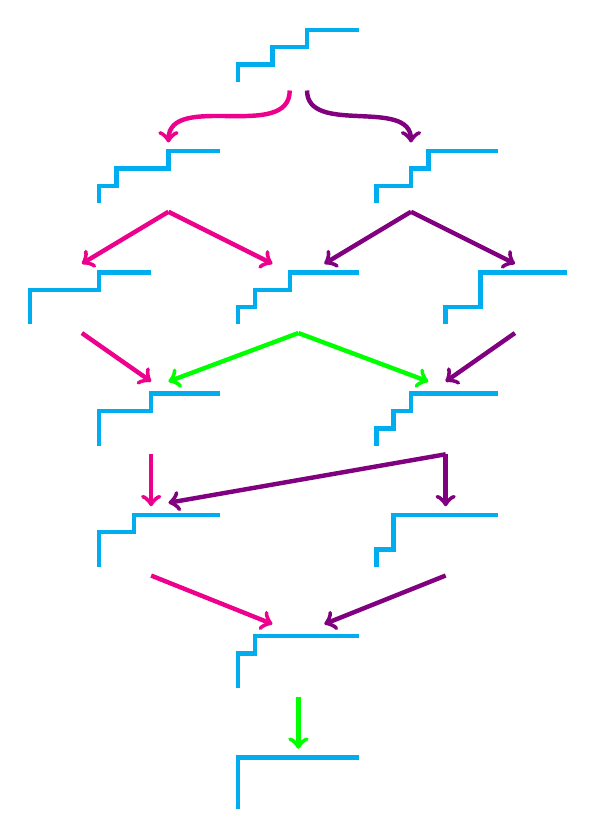
\begin{tikzpicture}[scale = 0.22]
    \draw [ultra thick, color = cyan] (0,0) -- (0,1)
        -- (0,2) -- (0,3) -- (1,3) -- (2,3) -- (3,3)
        -- (4,3) -- (5,3) -- (6,3) -- (7,3);

    \draw [ultra thick, color = cyan] (0,7) -- (0,8)
        -- (0,9) -- (1,9) -- (1,10) -- (2,10) -- (3,10)
        -- (4,10) -- (5,10) -- (6,10) -- (7,10);

    \draw [ultra thick, color = cyan] (-8,14) -- (-8,15)
        -- (-8,16) -- (-7,16) -- (-6,16) -- (-6,17) -- (-5,17)
        -- (-4,17) -- (-3,17) -- (-2,17) -- (-1,17);
        
    \draw [ultra thick, color = cyan] (8,14) -- (8,15)
        -- (9,15) -- (9,16) -- (9,17) -- (10,17)
        -- (11,17) -- (12,17) -- (13,17) -- (14,17)
        -- (15,17);

    \draw [ultra thick, color = cyan] (-8,21) -- (-8,22)
        -- (-8,23) -- (-7,23) -- (-6,23) -- (-5,23)
        -- (-5,24) -- (-4,24) -- (-3,24) -- (-2,24)
        -- (-1, 24);

    \draw [ultra thick, color = cyan] (8,21) -- (8,22)
        -- (9,22) -- (9,23) -- (10,23) -- (10,24) -- (11,24)
        -- (12,24) -- (13,24) -- (14,24) -- (15,24);

    \draw [ultra thick, color = cyan] (-12,28) -- (-12,29)
        -- (-12,30) -- (-11,30) -- (-10,30) -- (-9,30) -- (-8,30)
        -- (-8,31) -- (-7,31) -- (-6,31) -- (-5,31);

    \draw [ultra thick, color = cyan] (0,28) -- (0,29)
        -- (1,29) -- (1,30) -- (2,30) -- (3,30) -- (3,31)
        -- (4,31) -- (5,31) -- (6,31) -- (7,31);

    \draw [ultra thick, color = cyan] (12,28) -- (12,29)
        -- (13,29) -- (14,29) -- (14,30) -- (14,31) -- (15,31)
        -- (16,31) -- (17,31) -- (18,31) -- (19,31);

    \draw [ultra thick, color = cyan] (-8,35) -- (-8,36)
        -- (-7,36) -- (-7,37) -- (-6,37) -- (-5,37) -- (-4,37)
        -- (-4,38) -- (-3,38) -- (-2,38) -- (-1,38);

    \draw [ultra thick, color = cyan] (8,35) -- (8,36)
        -- (9,36) -- (10,36) -- (10,37) -- (11,37) -- (11,38)
        -- (12,38) -- (13,38) -- (14,38) -- (15,38);

    \draw [ultra thick, color = cyan] (0,42) -- (0,43)
        -- (1,43) -- (2,43) -- (2,44) -- (3,44) -- (4,44)
        -- (4,45) -- (5,45) -- (6,45) -- (7,45);

    \draw [->][out=-90,in=90, ultra thick] 
        [color=magenta](3,41.5) to (-4,38.5);
    \draw [->][color=magenta, ultra thick]
        (-4,34.5) to (-9,31.5);
    \draw [->][color=magenta, ultra thick]
        (-4,34.5) to (2,31.5);        
    \draw [->][color=magenta, ultra thick]
        (-9,27.5) to (-5,24.7);
    \draw [->][color=magenta, ultra thick]
        (-5,20.5) to (-5,17.5);
    \draw [->][color=magenta, ultra thick]
        (-5,13.5) to (2,10.7);

    \draw [->][color=green, ultra thick]
        (3.5,27.5) to (-4,24.7);
    \draw [->][color=green, ultra thick]
        (3.5,27.5) to (11,24.7);
    \draw [->][out=-90,in=90, ultra thick] 
        [color=green](3.5,6.5) to (3.5,3.5);

    \draw [->][out=-90,in=90, ultra thick]
        [color=violet](4,41.5) to (10,38.5);
    \draw [->][color=violet, ultra thick]
        (10,34.5) to (5,31.5);
    \draw [->][color=violet, ultra thick]
        (10,34.5) to (16,31.5);
    \draw [->][color=violet, ultra thick]
        (16,27.5) to (12,24.7);
    \draw [->][color=violet, ultra thick]
        (12,20.5) to (-4,17.7);
    \draw [->][color=violet, ultra thick]
        (12,20.5) to (12,17.5);
    \draw [->][color=violet, ultra thick]
        (12,13.5) to (5,10.7);

\end{tikzpicture}
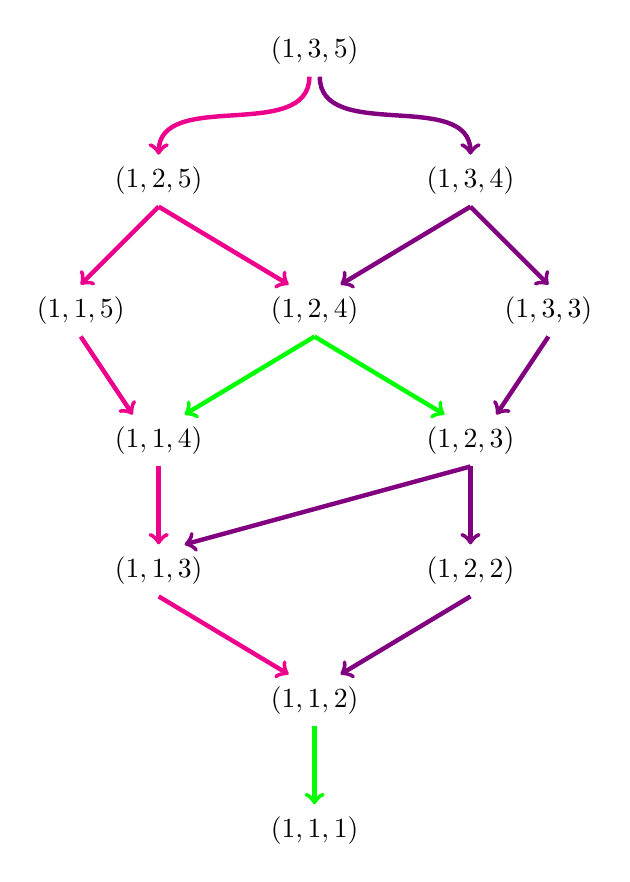
\begin{tikzpicture}[scale = 0.33]
    \node at (0,0) {$(1,1,1)$};

    \node at (0,5) {$(1,1,2)$};

    \node at (-6,10) {$(1,1,3)$};                
    \node at (6,10)  {$(1,2,2)$};

    \node at (-6,15) {$(1,1,4)$};
    \node at (6,15)  {$(1,2,3)$};

    \node at (-9,20) {$(1,1,5)$};
    \node at (0,20)  {$(1,2,4)$};
    \node at (9,20)  {$(1,3,3)$};

    \node at (-6,25) {$(1,2,5)$};
    \node at (6,25)  {$(1,3,4)$};

    \node at (0,30) {$(1,3,5)$};

    \draw [->][out=-90,in=90, ultra thick] 
        [color=magenta](-0.2,29) to (-6,26);
    \draw [->][color=magenta, ultra thick]
        (-6,24) to (-9,21);
    \draw [->][color=magenta, ultra thick]
        (-6,24) to (-1,21);        
    \draw [->][color=magenta, ultra thick]
        (-9,19) to (-7,16);
    \draw [->][color=magenta, ultra thick]
        (-6,14) to (-6,11);
    \draw [->][color=magenta, ultra thick]
        (-6,9) to (-1,6);

    \draw [->][color=green, ultra thick]
        (0,19) to (-5,16);
    \draw [->][color=green, ultra thick]
        (0,19) to (5,16);
    \draw [->][out=-90,in=90, ultra thick] 
        [color=green](0,4) to (0,1);

    \draw [->][out=-90,in=90, ultra thick]
        [color=violet](0.2,29) to (6,26);
    \draw [->][color=violet, ultra thick]
        (6,24) to (1,21);
    \draw [->][color=violet, ultra thick]
        (6,24) to (9,21);
    \draw [->][color=violet, ultra thick]
        (9,19) to (7,16);
    \draw [->][color=violet, ultra thick]
        (6,14) to (-5,11);
    \draw [->][color=violet, ultra thick]
        (6,14) to (6,11);
    \draw [->][color=violet, ultra thick]
        (6,9) to (1,6);

\end{tikzpicture}
~\\
~\\
\end{example}